%%%%%%%%%%%%%%%%%%%%%%%%%%%%%%%%%%%%%%%%%%%
%%%%%%%%%%%%%%%%%%%%%%%%%%%%%%%%%%%%%%%%%%%
%%%%%%%%%%%%%%% CHAPTER 05 %%%%%%%%%%%%%%%%

\section{Introdução aos comandos elétricos}

\frame{
\frametitle{Contextualização}
\begin{block}{}
\begin{itemize}
    \item O motor de um automóvel precisa ser acionado de alguma maneira.
    \item Fazemos isso usando \textbf{comandos elétricos}.
\end{itemize}
\end{block}
\centerline{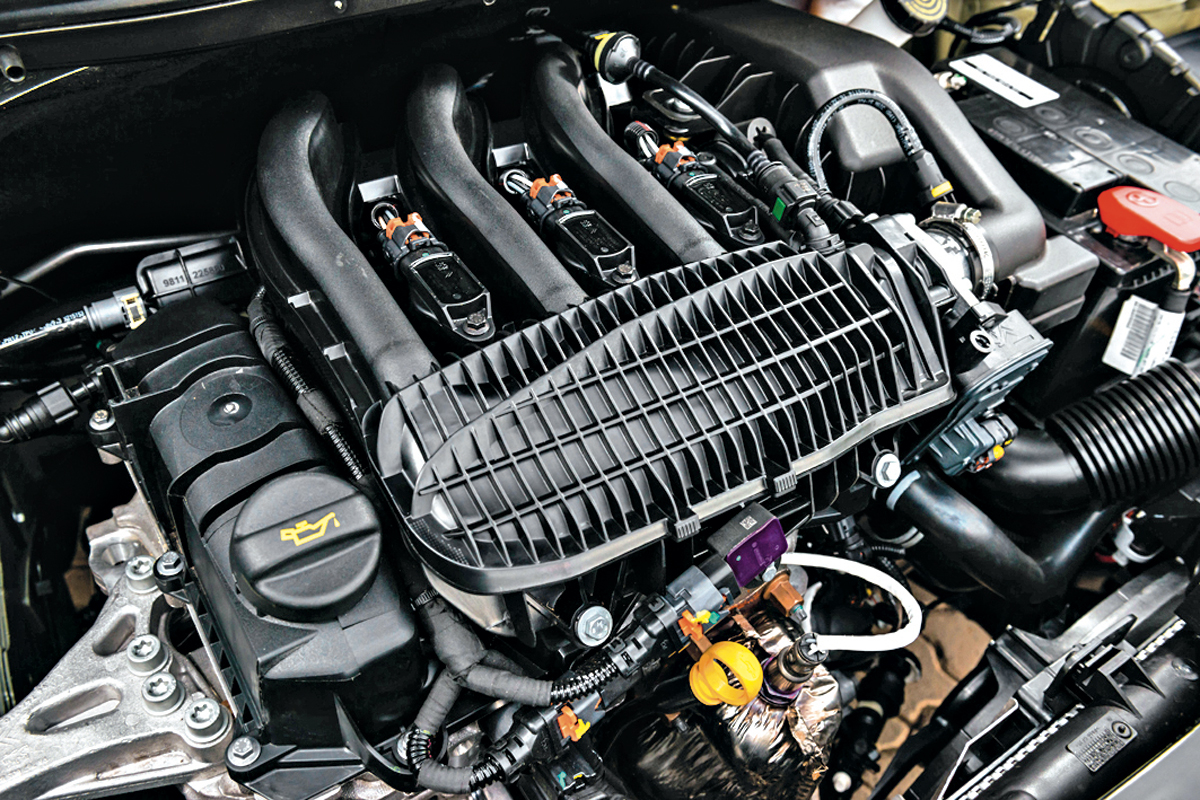
\includegraphics[width=0.75\linewidth]{Figuras/Ch05/fig1.jpg}}
}

\frame{
\frametitle{Circuitos}
\begin{block}{}
	Os comandos elétricos podem ser representados por um circuito geral que deve:
	\begin{itemize}
		\item Energizar o equipamento
		\item Proteger o equipamento
		\item Comandar o equipamento
	\end{itemize}
	Dizemos que os comandos elétricos têm por finalidade a \textbf{manobra} dos equipamentos elétricos.
\end{block}
\centerline{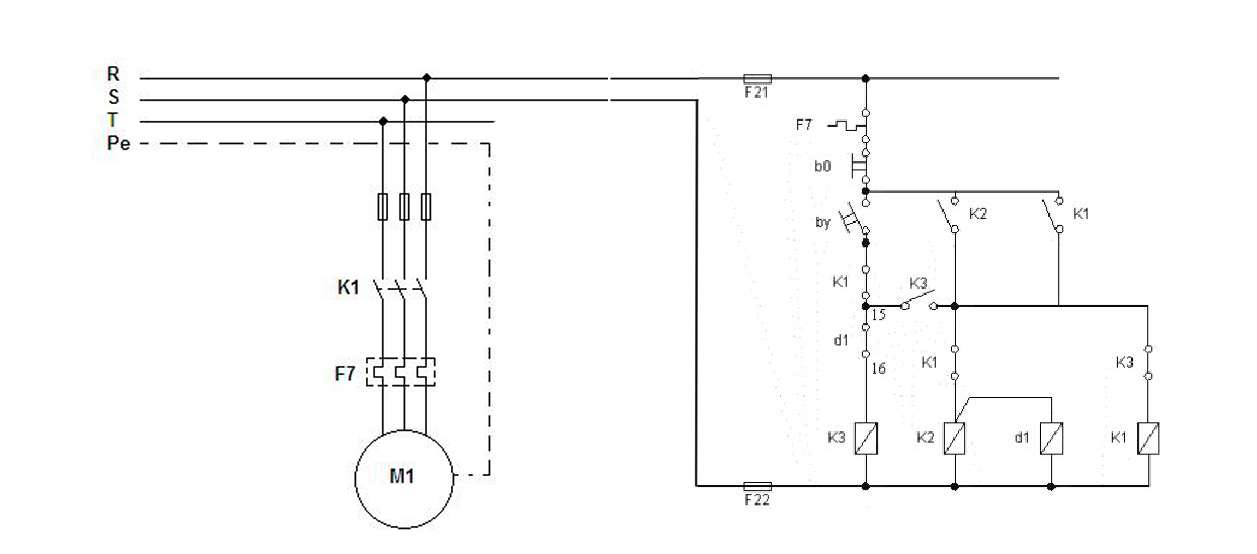
\includegraphics[height=0.45\textheight]{Figuras/Ch05/fig2.jpg}}
}

\frame{
\frametitle{Circuitos}
\begin{block}{}
	Esse circuito geral, por sua vez, pode ser separado em dois circuitos menores:
	\begin{itemize}
		\item Circuito de \textbf{força}
	\end{itemize}
	Este deve \textbf{energizar} e \textbf{proteger} o equipamento
\end{block}
\centerline{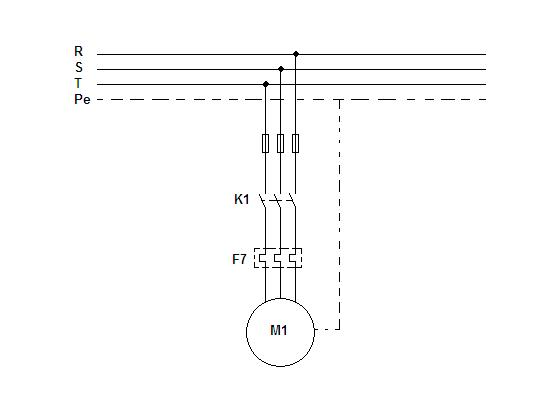
\includegraphics[width=0.6\linewidth]{Figuras/Ch05/fig3.jpg}}
}

\frame{
\frametitle{Circuitos}
\begin{block}{}
	\begin{itemize}
		\item Circuito de \textbf{comando}
	\end{itemize}
	Este deve \textbf{comandar} o equipamento
\end{block}
\centerline{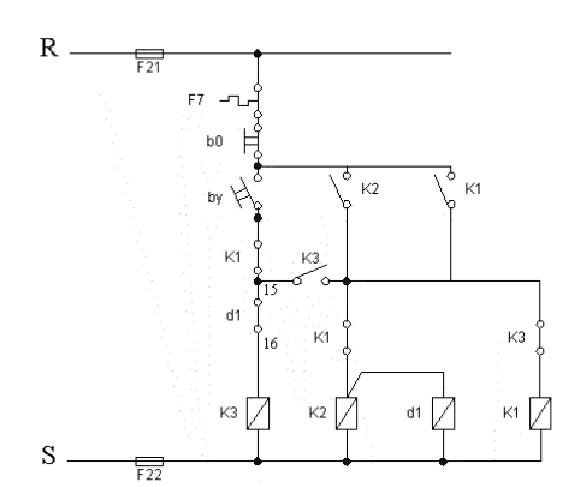
\includegraphics[width=0.6\linewidth]{Figuras/Ch05/fig4.jpg}}
}

\begin{frame}
\frametitle{Circuitos}
\begin{block}{Circuito de força}
	\begin{itemize}
		\item O circuito de força (ou de \textit{potência}) é geralmente \textbf{trifásico} e alimenta a carga principal apresentando, usualmente, correntes relativamente altas e, portanto, fios com grandes bitolas.
		\item É no circuito de força que estão presentes as demais \textbf{proteções} do equipamento de potência.
	\end{itemize}
\end{block}
\end{frame}

\begin{frame}
\frametitle{Circuitos}
\begin{block}{Circuito de comando}
	\begin{itemize}
		\item O circuito de comando é \textbf{independente} do circuito de potência, mesmo que frequentemente utilizem a mesma fonte de tensão.
		\item O circuito de comando deve \textbf{modificar o estado} do equipamento que desejamos utilizar.
		\item A \textbf{sinalização} (lâmpadas de liga/desliga, etc.) é realizada nessa parte do circuito principal.
	\end{itemize}
\end{block}
\end{frame}

\begin{frame}
\frametitle{Circuitos}
\begin{block}{}
	É importante separar o circuito principal em partes (força e comando) pois:
	\begin{itemize}
		\item Assim podemos controlar nosso equipamento com menos complicações.
		\item É mais fácil \textbf{identificar} e \textbf{resolver} quaisquer problemas que surjam.
		\item É mais \textbf{barato} e mais \textbf{seguro}, pois enquanto o equipamento geralmente precisa de correntes altas (e \textbf{perigosas}) os componentes utilizados para comandá-lo podem operar com correntes baixas, que podem usar fios mais finos (e mais \textbf{baratos}).
	\end{itemize}
\end{block}
\end{frame}

\begin{frame}{Exemplo \#01}
\begin{block}{Definição do problema}
	\begin{itemize}
		\item O dono de um sítio quer instalar um portão automático.
		\item O portão deve abrir quando alguém acionar um botão.
	\end{itemize}
\end{block}
\centerline{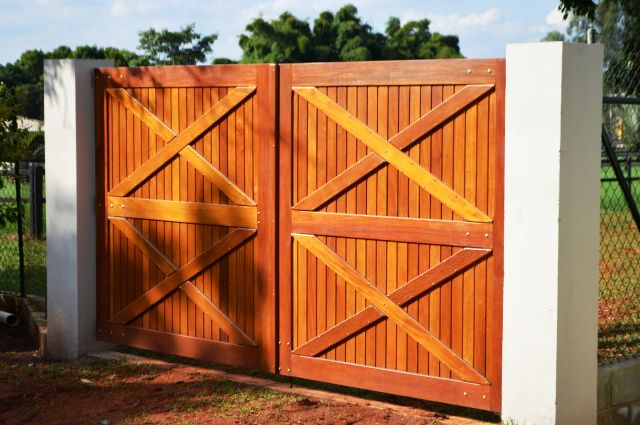
\includegraphics[width=0.7\linewidth]{Figuras/Ch05/fig5.jpg}}
\end{frame}

\begin{frame}{Exemplo \#01}
\begin{block}{Interpretação}
	\begin{itemize}
		\item O portão será aberto por um \textit{motor}.
		\item O motor será energizado e protegido por um \textit{circuito de potência}.
		\item Um \textit{botão} deverá acionar o motor.
	\end{itemize}
\end{block}
\end{frame}

\begin{frame}{Exemplo \#01}
\begin{block}{Perguntas}
	\begin{itemize}
		\item Como o botão aciona o motor?
		\item Como lidar com possíveis problemas elétricos?
		\item E se houver alguma coisa no caminho do portão enquanto ele abre? E se for uma pessoa? Vai se machucar?
	\end{itemize}
\end{block}
\end{frame}

\begin{frame}{Como o botão aciona o motor?}
\begin{block}{No circuito}
O botão pode ser representado por:
\end{block}

\medskip
\begin{center}
	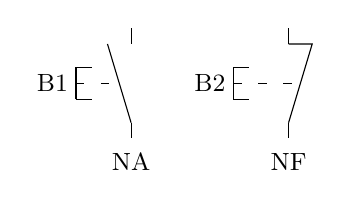
\begin{tikzpicture}
	\draw (-0.2,0.3) -- +(0.2,0) (-0.2,0.3) -- ++(0,0.4) -- +(0.2,0) (1.8,0.3) -- +(0.2,0) (1.8,0.3) -- ++(0,0.4) -- +(0.2,0);
	\draw[loosely dashed] (-0.2, 0.5) -- +(0.55,0) (1.8,0.5) -- +(0.85,0);
	\draw (0.5, 1) -- +(0,0.2) (0.5,0) -- +(0,-0.2);
	\draw (2,0) ++(0.5, 1) -- +(0,0.2) (2,0) ++(0.5,0) -- +(0,-0.2);
	\draw (0.5,0) -- +(-0.3,1) (2,0) ++(0.5,0) -- ++(0.3,1) -- +(-0.3,0);
	\node at (-0.5, 0.5) {\small B1};
	\node at (1.5, 0.5) {\small B2};
	\node at (0.5, -0.5) {\small NA};
	\node at (2.5, -0.5) {\small NF};
	\end{tikzpicture}
\end{center}

\vspace{-1em}

\begin{block}{}
Repare que há duas possibilidades de botão:
\begin{itemize}
	\item NA (normalmente aberto)
	
	O botão NA deixa o circuito \textbf{aberto} (corrente não consegue fluir) enquanto não for pressionado.
	\item NF (normalmente fechado)
	
	O botão NA deixa o circuito \textbf{fechado} (corrente pode fluir normalmente) enquanto não for pressionado.
\end{itemize}
\end{block}
\end{frame}


\begin{frame}{Como o botão aciona o motor?}
\begin{block}{No circuito}
	\begin{itemize}
	    \item Sabendo que as duas partes do nosso circuito (força e comando) são \textbf{separadas}, como podemos acionar a parte de força se o botão está na parte de comando e \textbf{não} há fios ligando as duas partes diretamente?
	    \item Aí entram os \textbf{contatores}.
	    \item Os contatores têm a função de, ao serem acionados por uma corrente baixa e segura, acionarem suas chaves (similares a botões, mas que não podem ser pressionados), estas, por sua vez, podem estar no circuito de força, pois possuem capacidade de operar com altas correntes.
	\end{itemize}
\end{block}
\end{frame}

\begin{frame}{Como o botão aciona o motor?}
\begin{block}{No circuito}
	O contator é representado por:
\end{block}

\vspace{1cm}

\noindent
\begin{minipage}{0.45\linewidth}
	\centering
	\begin{tikzpicture}
		\draw[loosely dashed] (0, 0.5) -- (1.5,0.5);
		
		\draw[fill=white, draw=white] (0.2,-0.2) rectangle (0.5,1.2) (1,0) ++(0.5,-0.2) rectangle +(0.3,1.4);
		
		\draw (0.5, 1) -- +(0,0.2) (0.5,0) -- +(0,-0.2);
		\draw (1,0) ++(0.5, 1) -- +(0,0.2) (1,0) ++(0.5,0) -- +(0,-0.2);
		\draw (0.5,0) -- +(-0.3,1) (1,0) ++(0.5,0) -- ++(0.3,1) -- +(-0.3,0);
		\node at (-0.25, 0.5) {\small K1};
	
	\end{tikzpicture}

	\noindent No diagrama de força
\end{minipage}
\hfill
\begin{minipage}{0.45\linewidth}
	\centering
	\vspace{-1.15cm}
	\begin{tikzpicture}
		\draw[loosely dashed] (-.75,0.5) -- (1.5,0.5);
		\draw[fill=white, draw=white] (0.2,-0.2) rectangle ++(0.3,1.4) ++(1,0) ++(0.5,-0.2) rectangle +(0.3,1.4);
		
		\draw (-2,0.25) ++(0.5, 0.5) -- +(0,0.2) (-2,0.25) ++(0.5,0) -- +(0,-0.2);
		\draw (-2,0.25) ++(0,0) rectangle +(1,0.5);
		\node at (-2.25, 0.5) {\small K1};
		
		\draw (0.5, 1) -- +(0,0.2) (0.5,0) -- +(0,-0.2);
		\draw (1,0) ++(0.5, 1) -- +(0,0.2) (1,0) ++(0.5,0) -- +(0,-0.2);
		\draw (0.5,0) -- ++(-0.3,1) (1,0) ++(0.5,0) -- ++(0.3,1) -- +(-0.3,0);
	\end{tikzpicture}
	
	\noindent No diagrama de comando
\end{minipage}
\end{frame}


\begin{frame}{Como o botão aciona o motor?}
\begin{block}{No circuito}
\begin{itemize}
	\item A \textbf{bobina do contator} é representada pela caixa retangular, é ela que acionamos no circuito de comando.
\end{itemize}
\end{block}
\begin{center}
	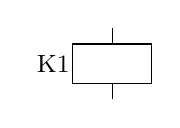
\begin{tikzpicture}
	\draw (0.5, 0.5) -- +(0,0.2) (0.5,0) -- +(0,-0.2);
	\draw (0,0) rectangle (1,0.5);
	\node at (-0.25, 0.25) {\small K1};
	\end{tikzpicture}
\end{center}
\begin{block}{}
\begin{itemize}
	\item A simbologia das \textbf{chaves do contator} é apresentada abaixo.
\end{itemize}
\end{block}
\begin{center}
	\begin{tikzpicture}
	\draw[loosely dashed] (0, 0.5) -- (1.5,0.5);
	\draw[fill=white, draw=white] (0.2,-0.2) rectangle (0.5,1.2) (1,0) ++(0.5,-0.2) rectangle +(0.3,1.4);
	\draw (0.5, 1) -- +(0,0.2) (0.5,0) -- +(0,-0.2);
	\draw (1,0) ++(0.5, 1) -- +(0,0.2) (1,0) ++(0.5,0) -- +(0,-0.2);
	\draw (0.5,0) -- +(-0.3,1) (1,0) ++(0.5,0) -- ++(0.3,1) -- +(-0.3,0);
	\node at (-0.25, 0.5) {\small K1};
	\end{tikzpicture}
\end{center}
\begin{block}{}
\begin{itemize}
	\item A primeira é do tipo NA e a segunda NF, com funcionamento idêntico aos botões que vimos anteriormente. O tracejado indica que ambas pertencem ao mesmo contator (K1).
\end{itemize}
\end{block}
\end{frame}


\begin{frame}{Como o botão aciona o motor?}
\begin{block}{No circuito}
	\begin{itemize}
		\item O botão pode ser representado por B1 no diagrama e o contator que liga o motor por K1.
	\end{itemize}
\end{block}
\centerline{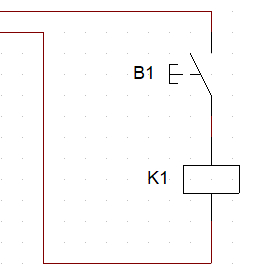
\includegraphics[width=0.4\linewidth]{Figuras/Ch05/fig6.jpg}}
\end{frame}


\begin{frame}{Como o botão aciona o motor?}
\begin{block}{No circuito}
	\begin{itemize}
		\item O motor está representado pelo círculo com a letra M dentro. L1, L2 e  L3 se referem às linhas de alimentação (sistema trifásico). 
		\item Também podemos usar as letras R, S e T.
	\end{itemize}
\end{block}
\centerline{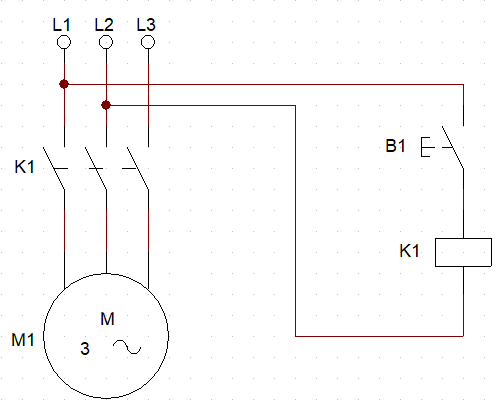
\includegraphics[height=0.6\textheight]{Figuras/Ch05/fig7.jpg}}
\end{frame}


\begin{frame}{Como o botão aciona o motor?}
\begin{block}{No circuito}
	\begin{itemize}
		\item Se pressionarmos o botão B1 o circuito se fechará e ativará a bobina do contator K1, o qual possui chaves no circuito de força que vão ligar o motor.
	\end{itemize}
\end{block}
\centerline{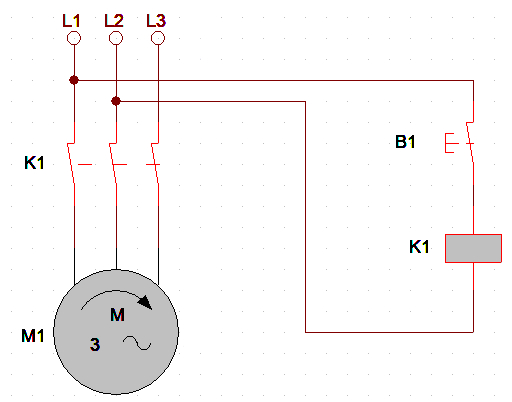
\includegraphics[width=0.4\linewidth]{Figuras/Ch05/fig8.jpg}}
\begin{block}{}
	\begin{itemize}
		\item Repare que o portão só se moverá significativamente se mantivermos o botão pressionado, caso contrário ele vai meramente dar um solavanco.
	\end{itemize}
\end{block}
\end{frame}

\begin{frame}{Exemplo \#01}
\begin{block}{Perguntas}
	\begin{itemize}
		\item Como o botão aciona o motor? \checkmark
		\item Como lidar com possíveis problemas elétricos?
		\item E se houver alguma coisa no caminho do portão enquanto ele abre? E se for uma pessoa? Vai se machucar?
	\end{itemize}
\end{block}
\end{frame}

\begin{frame}{Como lidar com possíveis problemas elétricos?}
\begin{block}{Curto-circuito}
    \begin{itemize}
        \item O \textbf{curto-circuito} é uma possibilidade nas instalações elétricas e pode queimar os equipamentos, portanto, como a instalação de um motor $ + $ contator não é algo barato, queremos protegê-la.
        \item Para proteger contra curtos podemos usar \textbf{fusíveis}, que são componentes relativamente baratos em comparação com o motor ou contator.
        \item Uma vez queimado o fusível deve ser trocado.
        \item O fusível pode ser representado por um retângulo em pé cortado ao meio por um fio.
    \end{itemize}
\end{block}
\begin{center}
	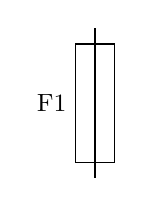
\begin{tikzpicture}
		\draw (0,0) rectangle (0.5,1.5);
		\draw (0.25, -0.2) -- (0.25,1.7);
		\node at (-0.3, 0.75) {\small F1};
	\end{tikzpicture}
\end{center}
\end{frame}

\begin{frame}{Como lidar com possíveis problema elétricos?}
\begin{block}{Fusíveis}
	\begin{itemize}
		\item Instalamos um fusível para cada fase distinta em um circuito, além de separarmos os fusíveis para o circuito de comando e o de potência.
	\end{itemize}
\end{block}
\centerline{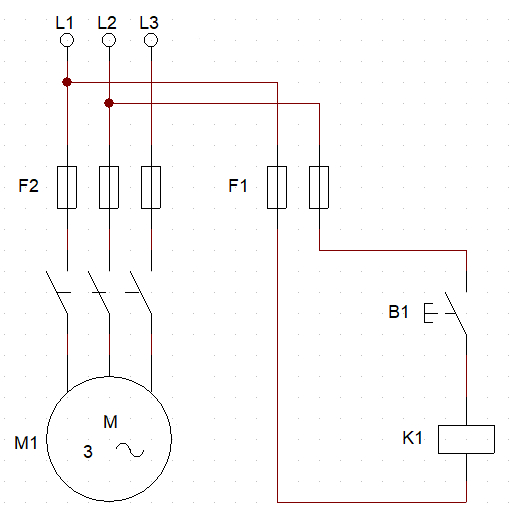
\includegraphics[height=0.6\textheight]{Figuras/Ch05/fig9.jpg}}
\end{frame}

\begin{frame}{Como lidar com possíveis problema elétricos?}
\begin{minipage}{0.45\linewidth}
	\centering
	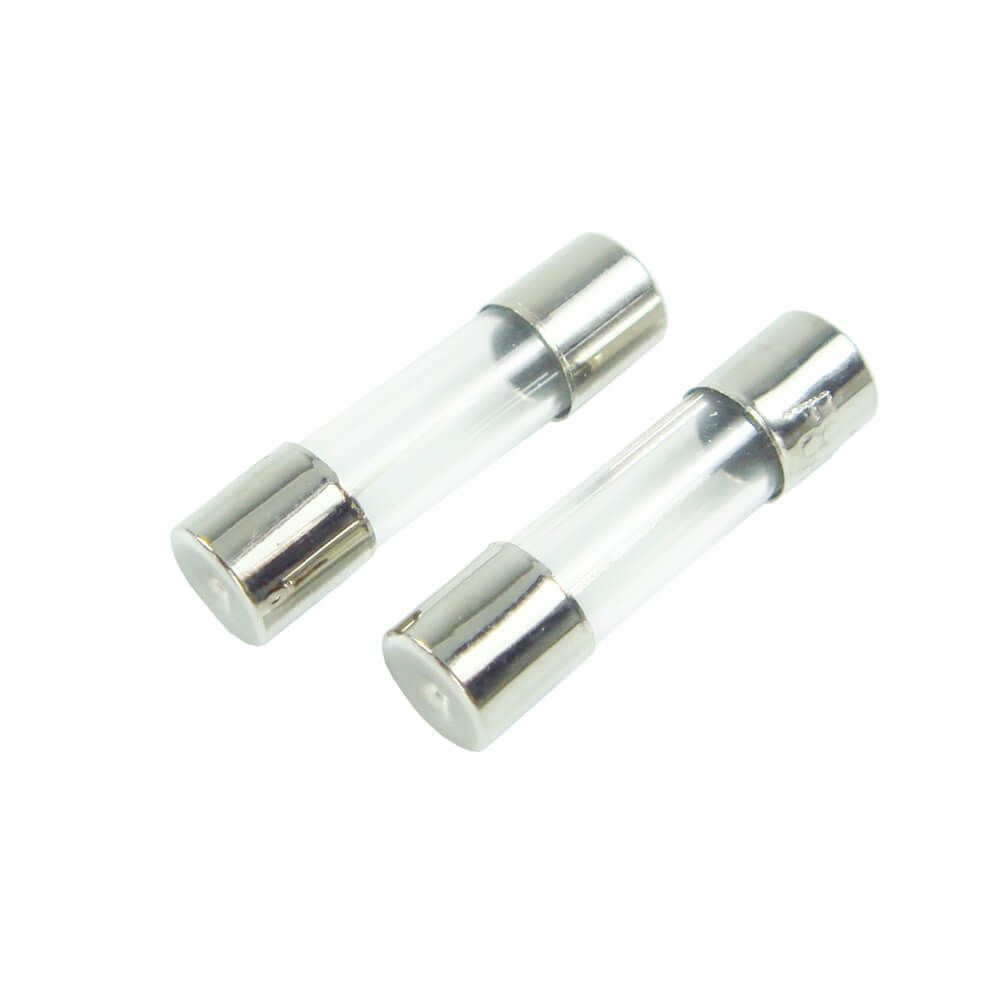
\includegraphics[width=\linewidth]{Figuras/Ch05/fig10.jpg}
\end{minipage}
\hfill
\begin{minipage}{0.45\linewidth}
	\centering
	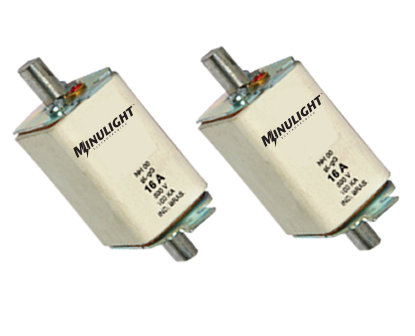
\includegraphics[width=\linewidth]{Figuras/Ch05/fig11.png}
\end{minipage}
\end{frame}

\begin{frame}{Como lidar com possíveis problemas elétricos?}
\begin{block}{Sobrecarga}
    \begin{itemize}
        \item A \textbf{sobrecarga} é um problema corriqueiro em instalações elétricas, ocorre quando a alimentação de energia dá picos de corrente, isso pode danificar equipamentos se não for remediado com certa urgência.
        \item Os \textbf{disjuntores} são capazes de proteger contra esse tipo de problema e também contra curtos. Eles não são tão baratos quanto os fusíveis mas podem ser religados, não necessitando serem trocados.
        \item A simbologia dos disjuntores de um motor é apresentada abaixo.
    \end{itemize}
\end{block}
\centerline{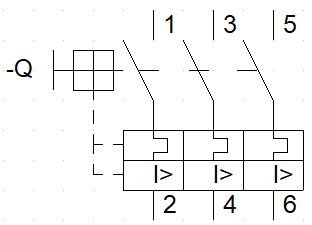
\includegraphics[height=0.3\textheight]{Figuras/Ch05/fig12.jpg}}
\end{frame}

\begin{frame}{Como lidar com possíveis problemas elétricos?}
\begin{block}{Disjuntor}
	\begin{itemize}
		\item O princípio de proteção contra sobrecargas de um disjuntor termomagnético é a \textbf{lâmina bimetálica}.
	\end{itemize}
\end{block}
	\begin{center}
		\begin{tikzpicture}
			\fill[pattern=north east lines] (0,0) rectangle +(-0.5,2);
			\draw (0,0) -- (0,2);
			\draw (0,1.2) -- ++(3,0) -- ++(0,-0.2) -- +(-3,0) (0,0.8) -- ++(3,0) -- +(0,0.2);
			\fill[pattern=north west lines] (0,0.8) rectangle +(3,0.2);
			\node at (1.5,1.4) {\small A};
			\node at (1.5,0.6) {\small B};
			\node(A) at (2,0) {};
			\node(B) at (2,2) {};
			\draw[->,>=Latex] (A) edge[bend right] (B);
		\end{tikzpicture}
	\end{center}
\begin{block}{}
	\begin{itemize}
		\item A e B são metais com coeficientes de dilatação térmica diferentes, então, como a corrente passando pelo dispositivo produz \textbf{calor} \textbf{proporcionalmente} à sua intensidade, quando a lâmina aquece acima de um limite, uma de suas partes \textbf{dilata mais} do que a outra e ela se dobra, \textbf{abrindo} o circuito.
	\end{itemize}
\end{block}
\end{frame}

\begin{frame}[fragile]{Como lidar com possíveis problemas elétricos?}
\begin{block}{Disjuntor}
	\begin{itemize}
		\item A proteção contra curtos do disjuntor termomagnético funciona usando o princípio da \textbf{indução eletromagnética}.
	\end{itemize}
\end{block}
	\begin{minipage}{0.45\linewidth}
		\centering
		\scalebox{0.95}{
			\begin{tikzpicture}
			
			\def\coil#1{
				{-2.5mm * cos(\t * pi r)+14},
				{0.15 * (2*#1 + \t) + 0.1*sin(\t * pi r)+0.67}
			}
			
			\foreach \n in {1,2} {
				\draw[domain={0:1},smooth,variable=\t,samples=15]
				plot (\coil{\n}); 
			}
			
			\draw[domain={0:0.5},smooth,variable=\t,samples=15] plot (\coil{3});
			
			% Draw the rectangle
			\filldraw[fill=white,draw=black] (0.3, 0) rectangle (0.7, 1.5);
			
			%	coil in front of the rectangle
			\foreach \n in {1,2} {
				\draw[domain={1:2},smooth,variable=\t,samples=15]
				plot (\coil{\n});
			}
			
			\draw[domain={1.5:2},smooth,variable=\t,samples=15] plot (\coil{0});
			
			
			\draw (-1,0.5) -- (0.5,0.5) -- +(0,0.3) (-1,2) -- (0.5,2) -- (0.5,1.75);
			\draw[->,>=Latex] (-1,2.1) -- +(0.5,0) node[above] {$ i $};
			\draw[->,>=Latex] (-1,0.1) -- +(0.5,0) node[above] {$ i $};
			\draw (0.5, 0.3) -- +(1,0.5) node[right] {barra metálica};
			\draw (-1,0) -- (0,0)
			node[circle,fill=black,inner sep=1] {} -- (1,0) node[circle,fill=black,inner sep=1] {} -- (2,0);
			\end{tikzpicture}}
	\end{minipage}
	\hfill
	\begin{minipage}{0.45\linewidth}
		\centering
		\scalebox{0.95}{
			\begin{tikzpicture}
			\def\coil#1{
				{-2.5mm * cos(\t * pi r)+14},
				{0.15 * (2*#1 + \t) + 0.1*sin(\t * pi r)+0.67}
			}
			\foreach \n in {1,2} {
				\draw[domain={0:1},smooth,variable=\t,samples=15]
				plot (\coil{\n}); 
			}
			\draw[domain={0:0.5},smooth,variable=\t,samples=15] plot (\coil{3});
			\filldraw[fill=white,draw=black] (0.3, 0.35) rectangle (0.7, 1.85);
			\foreach \n in {1,2} {
				\draw[domain={1:2},smooth,variable=\t,samples=15]
				plot (\coil{\n});
			}
			\draw[domain={1.5:2},smooth,variable=\t,samples=15] plot (\coil{0});
			\draw (-1,0.5) -- (0.5,0.5) -- +(0,0.3) (-1,2) -- (0.5,2) -- (0.5,1.85);
			\draw[->,>=Latex] (-1,2.1) -- +(0.5,0) node[above] {$ i^\prime $};
			\draw (-1,0) -- (0,0)
			node[circle,fill=black,inner sep=1] {} -- (1,0.5) node[circle,fill=black,inner sep=1] {} (1,0) -- (2,0);
			\end{tikzpicture}}
	\end{minipage}
	\medskip
	\begin{block}{}
	\begin{itemize}
		\item Dentro do disjuntor existe um conjunto bobina-barra metálica. Essa barra fica acoplada à uma chave NF que, quando aberta, \textbf{bloqueia} a passagem de corrente para o circuito. Quando ocorre alguma \textbf{variação brusca} de corrente a bobina ganha um campo magnético que \textbf{puxa} a barra metálica, \textbf{abrindo} a chave e fazendo \textbf{cessar} o fluxo de corrente no circuito.
	\end{itemize}
	
\end{block}
\end{frame}

\begin{frame}{Como lidar com possíveis problemas elétricos?}
\begin{minipage}{0.45\linewidth}
	\centering
	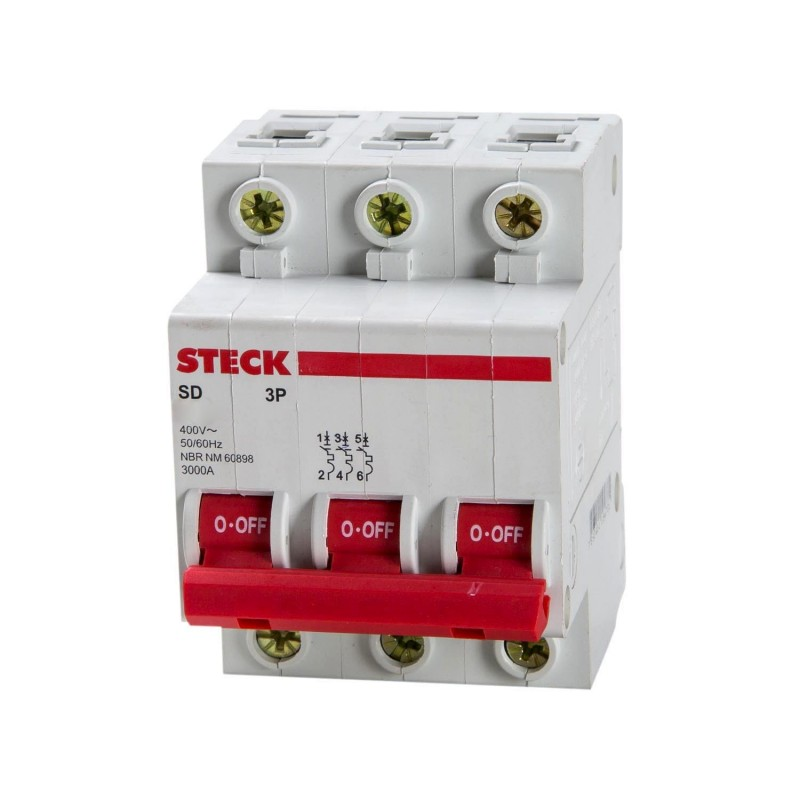
\includegraphics[width=\linewidth]{Figuras/Ch05/fig13.jpg}
\end{minipage}
\hfill
\begin{minipage}{0.45\linewidth}
	\centering
	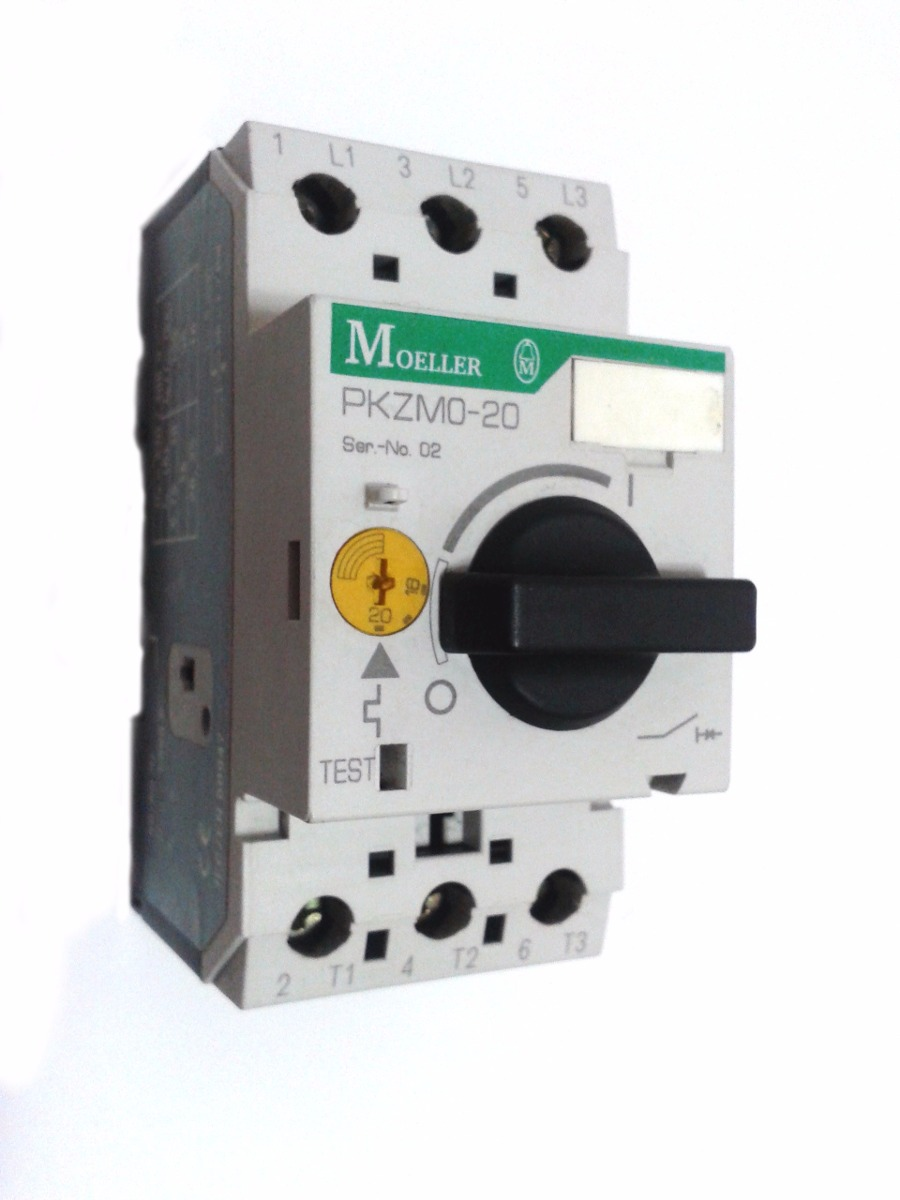
\includegraphics[width=\linewidth]{Figuras/Ch05/fig14.jpg}
\end{minipage}
\end{frame}

\begin{frame}{Como lidar com possíveis problemas elétricos?}
\begin{block}{Relé térmico ou de sobrecarga}
    \begin{itemize}
        \item O relé térmico é outro dispositivo que conta com \textbf{proteção de sobrecarga}, usando o mesmo princípio que o disjuntor (lâmina bimetálica). Ele também pode ser rearmado.
        \item O \textbf{relé térmico} é usado somente para proteção do \textbf{equipamento} ligado ao circuito de força (motor do portão no nosso exemplo), ao \textbf{contrário} do disjuntor, que pode ser usado para a proteção de \textbf{todo} o circuito. No nosso exemplo, o motor que abre o portão pode ser protegido com um relé térmico.
        \item A simbologia do relé térmico é apresentada abaixo.
    \end{itemize}
\end{block}
\begin{minipage}{0.45\linewidth}
	\centering
	\begin{tikzpicture}[scale=0.9]
		\draw (0.5,1) rectangle (2.8,2);
		\node at (0.,1.5) {FT};
		\draw (1,2.5) -- ++(0,-0.7) -- ++(-0.3,0) -- ++(0,-0.6) -- ++(0.3,0) -- ++(0,-0.7); 
		\draw (0.8,0) ++(1,2.5) -- ++(0,-0.7) -- ++(-0.3,0) -- ++(0,-0.6) -- ++(0.3,0) -- ++(0,-0.7);
		\draw (1.6,0) ++(1,2.5) -- ++(0,-0.7) -- ++(-0.3,0) -- ++(0,-0.6) -- ++(0.3,0) -- ++(0,-0.7);
	\end{tikzpicture}
	
	\vspace{-0.5cm}
	No diagrama de força
\end{minipage}
\hfill
\begin{minipage}{0.45\linewidth}
	\centering
	\begin{tikzpicture}[scale=1.1]
	\draw (-0.5,0.4) -- ++(0.2,0) -- ++(0,0.1) -- ++(0.2,0) -- ++(0,-0.1) -- (0.37, 0.4);
	\draw (1.6,0.4) -- ++(0.2,0) -- ++(0,0.1) -- ++(0.2,0) -- ++(0,-0.1) -- (2.63, 0.4);
	\fill (-0.5,0.5) -- ++(0,-0.1) -- ++(0.2,0) -- cycle;
	\fill (1.6,0.5) -- ++(0,-0.1) -- ++(0.2,0) -- cycle;
	\draw (0.5, 1) -- +(0,0.2) (0.5,0) -- +(0,-0.2);
	\draw (2,0) ++(0.5, 1) -- +(0,0.2) (2,0) ++(0.5,0) -- +(0,-0.2);
	\draw (0.5,0) -- +(-0.3,1) (2,0) ++(0.5,0) -- ++(0.3,1) -- +(-0.3,0);
	\node at (-0.8, 0.5) {\small FT};
	\node at (1.3, 0.5) {\small FT};
	\end{tikzpicture}
	
	\vspace{0.35cm}
	No diagrama de comando
\end{minipage}
\end{frame}


\begin{frame}{Exemplo \#01}
\begin{block}{Perguntas}
	\begin{itemize}
		\item Como o botão aciona o motor? \checkmark
		\item Como lidar com possíveis problemas elétricos? \checkmark
		\item E se houver alguma coisa no caminho do portão enquanto ele abre? E se for uma pessoa? Vai se machucar?
	\end{itemize}
\end{block}
\end{frame}


\begin{frame}{E se houver alguma coisa no caminho do portão enquanto ele abre?}
\begin{block}{Sinalização}
	A fim de proteger o operador do equipamento e possíveis vítimas de acidentes podemos utilizar \textbf{sinalizadores}. Eles podem ser:
	\begin{itemize}
		\item Visuais
		\item Sonoros
	\end{itemize}
\end{block}
\end{frame}

\begin{frame}{E se houver alguma coisa no caminho do portão enquanto ele abre?}
\begin{block}{Sinalização}
	Os sinalizadores geralmente informam:
	\begin{itemize}
		\item Se o equipamento está \textbf{ligado} ou \textbf{desligado}
	\end{itemize}
\end{block}
\centerline{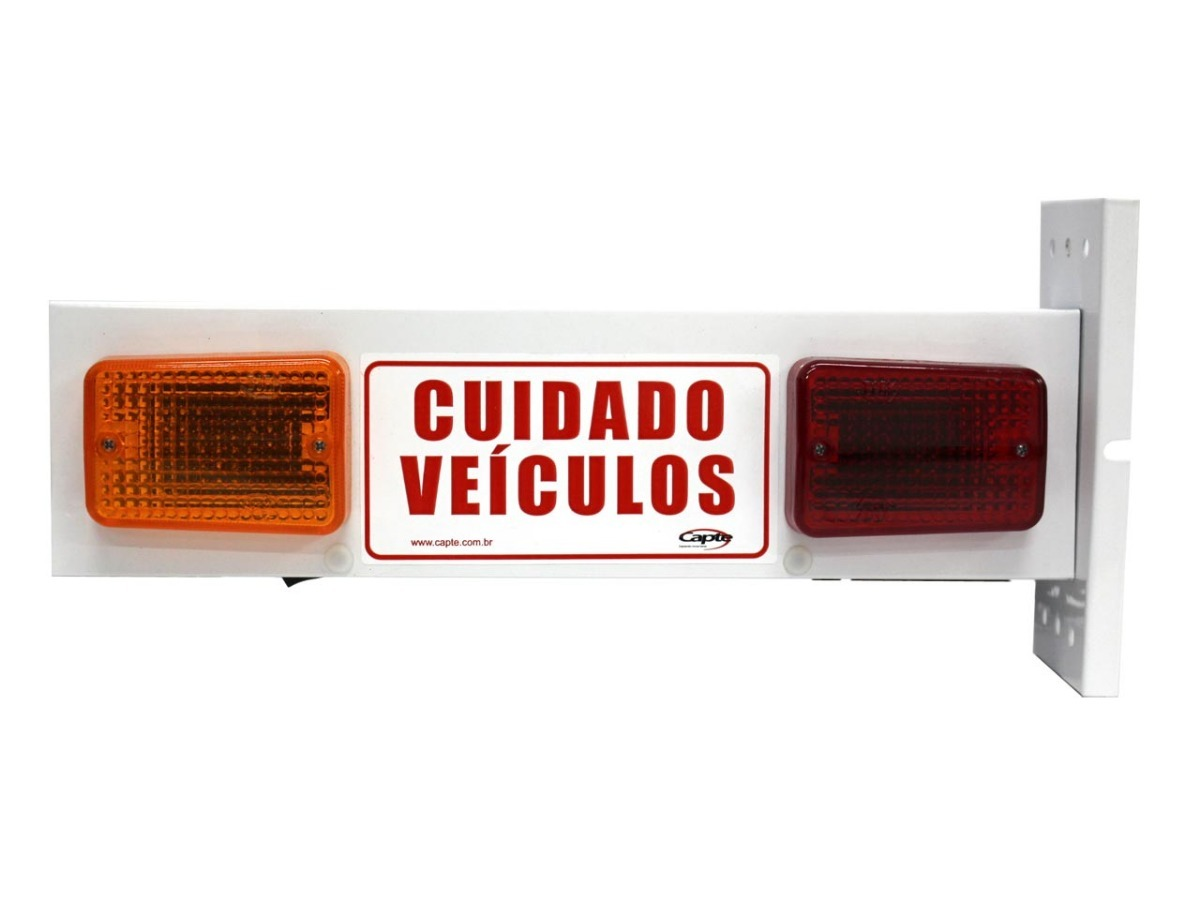
\includegraphics[width=0.7\linewidth]{Figuras/Ch05/fig15.jpg}}
\end{frame}

\begin{frame}{E se houver alguma coisa no caminho do portão enquanto ele abre?}
\begin{block}{Sinalização}
	\begin{itemize}
		\item Se houve \textbf{falha}
	\end{itemize}
\end{block}
\medskip
\centerline{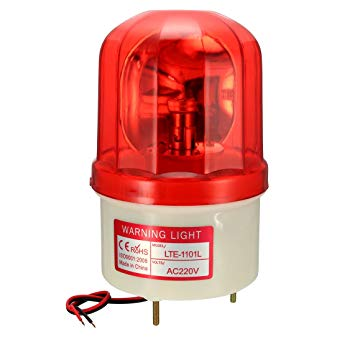
\includegraphics[width=0.4\linewidth]{Figuras/Ch05/fig16.jpg}}
\end{frame}

\begin{frame}{E se houver alguma coisa no caminho do portão enquanto ele abre?}
\begin{block}{Sinalização}
	\begin{itemize}
		\item Se há alguma \textbf{emergência}
	\end{itemize}
\end{block}
\medskip
\centerline{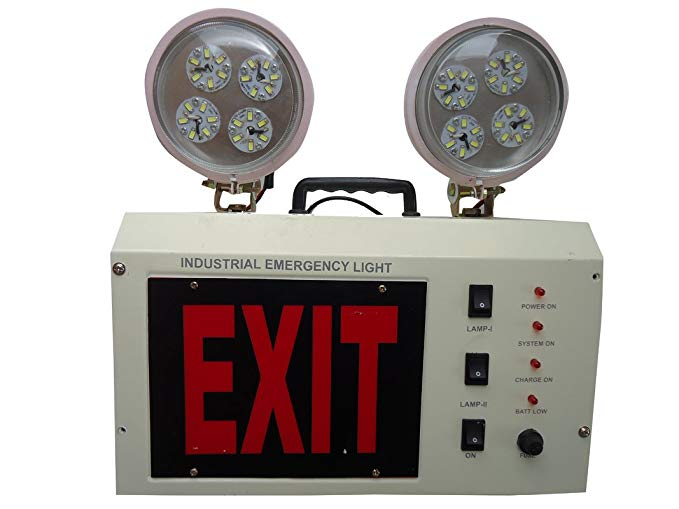
\includegraphics[width=0.5\linewidth]{Figuras/Ch05/fig17.jpg}}
\end{frame}



\begin{frame}{E se houver alguma coisa no caminho do portão enquanto ele abre?}
\begin{block}{Sinalização visual}
\begin{itemize}
    \item A sinalização visual pode ser feita por \textbf{lâmpadas} ou \textbf{LED's}.
    \item Esse tipo de sinalização é mais comum pois é mais \textbf{simples}, \textbf{barata} e \textbf{eficiente}.
    \item A simbologia da sinalização visual é apresentada abaixo.
\end{itemize}
\end{block}
\centerline{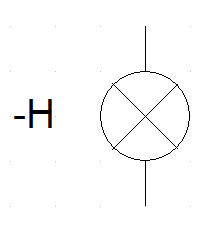
\includegraphics[width=0.3\linewidth]{Figuras/Ch05/fig18.jpg}}
\end{frame}


\begin{frame}{E se houver alguma coisa no caminho do portão enquanto ele abre?}
\begin{block}{Sinalização sonora}
\begin{itemize}
    \item A sinalização sonora é mais comum quando o ambiente é \textbf{amplo} e/ou \textbf{dividido em cômodos}.
    \item Embora seja menos comum na indústria temos vários exemplos na vida prática.
\end{itemize}
\end{block}
\centerline{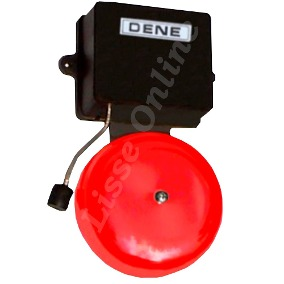
\includegraphics[width=0.4\linewidth]{Figuras/Ch05/fig19.jpg}}
\end{frame}


\begin{frame}{E se houver alguma coisa no caminho do portão enquanto ele abre?}
\centerline{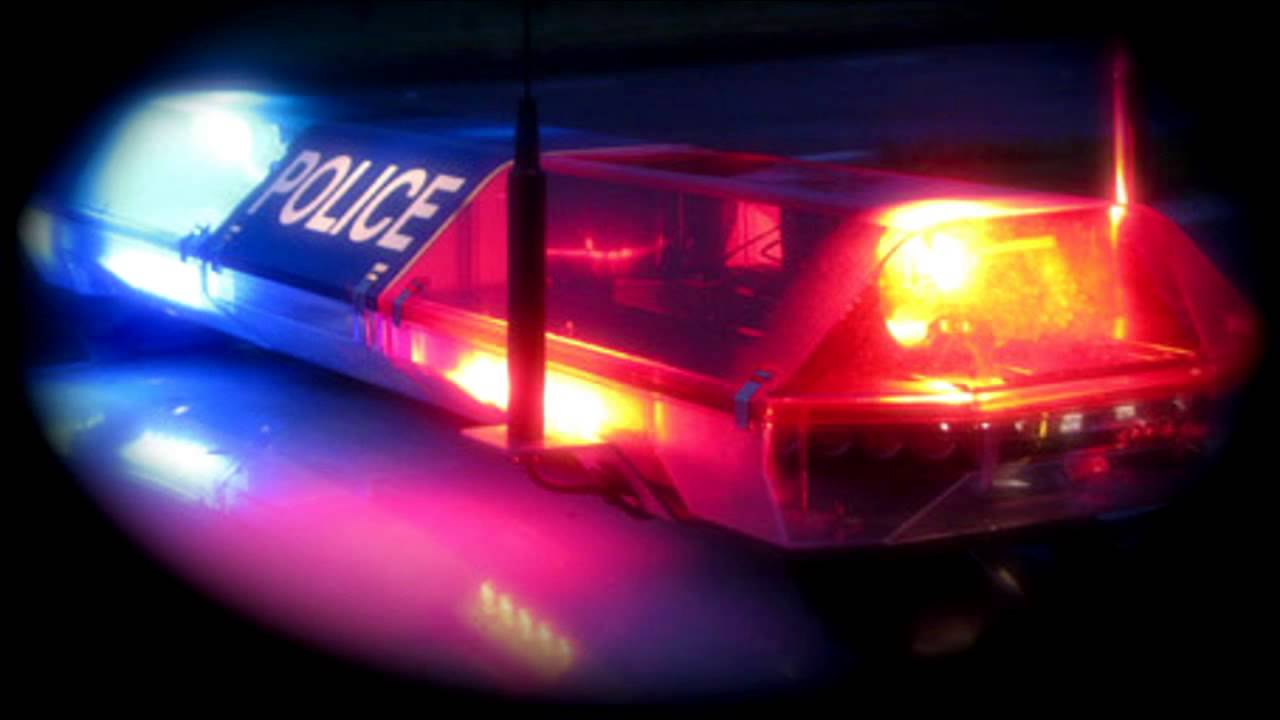
\includegraphics[width=\linewidth]{Figuras/Ch05/fig20.jpg}}
\end{frame}



\begin{frame}{E se houver alguma coisa no caminho do portão enquanto ele abre?}
\begin{block}{Sinalização visual}
	A sinalização sonora possui quatro símbolos diferentes, um para cada tipo de sinal. Os quatro símbolos são apresentados abaixo, sendo nomeados, da esquerda pra direita:
	
	\begin{itemize}
		\item Sinaleira
		\item Buzina
		\item Sirene
		\item Corneta
	\end{itemize}
	
\end{block}

\medskip

\centerline{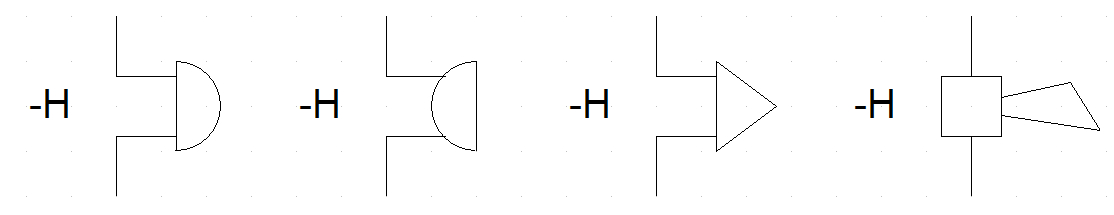
\includegraphics[width=0.8\linewidth]{Figuras/Ch05/fig21.jpg}}
\end{frame}

%\begin{frame}{Exemplo \#01}
%\begin{block}{Perguntas}
%	\begin{itemize}
%		\item Como o botão aciona o motor? \checkmark
%		\item Como lidar com possíveis problemas elétricos? \checkmark
%		\item E se houver alguma coisa no caminho do portão enquanto ele abre? E se for uma pessoa? Vai se machucar? \checkmark
%	\end{itemize}
%	Com nossas três perguntas iniciais respondidas, pode parecer que acabamos.
%	A pergunta que surge agora é:
%	\begin{itemize}
%		\item Como fechamos o portão?
%	\end{itemize}
%\end{block}
%\end{frame}

\frame{
	\frametitle{Exercícios}
	\begin{block}{}
		01. Descrever os componentes utilizados em um circuito de sinaleira de escola. A sinaleira deve ser acionada manualmente pelo operador.
		
		\vspace{0.5cm}
		
		02. Esboçar o circuito da sinaleira.
	\end{block}
}

\section*{Referências}
\frame{
	\frametitle{Referências e Exercícios Complementares}
	\begin{itemize}
		\item FILHO, João Mamede. Instalações Elétricas Industriais, 6 ed. Rio de Janeiro, LTC, 2001.
	\end{itemize}
	%\centering{\alert{Página 546 - \textbf{Capítulo 6}}} \\
	%\centering{\alert{Lista de exercícios 01}}
}